\documentclass[10pt,a4paper]{article}
\usepackage[italian]{babel}
\addto\captionsitalian{\renewcommand{\abstractname}{Abstract}}
\usepackage[utf8]{inputenc}
\usepackage[T1]{fontenc}
\usepackage{lmodern,microtype}
\usepackage{amsmath,amssymb,mathtools, amsthm}
\usepackage{graphicx,booktabs,array}
\usepackage{geometry,caption,pdflscape,float}
\usepackage{xcolor,hyperref,fancyhdr}
\geometry{margin=22mm,headheight=14pt}
\graphicspath{{report_assets/}}
\definecolor{deepblue}{HTML}{17324D}
\definecolor{teal}{HTML}{0F766E}
\hypersetup{colorlinks=true,linkcolor=deepblue,urlcolor=teal}
\captionsetup{font=small,labelfont=bf}
\pagestyle{fancy}
\fancyhf{}
\fancyhead[L]{\small Completion delle feature Breast Cancer}
\fancyhead[R]{\small Report sperimentale}
\fancyfoot[C]{\thepage}
\setlength{\parskip}{4pt}
\setlength{\parindent}{0pt}
\newcommand{\Obs}{\mathcal O}
\newcommand{\Hidden}{\mathcal H}
\newcommand{\RMSE}{\operatorname{RMSE}}
\newcommand{\MAE}{\operatorname{MAE}}
\newcommand{\C}{\mathcal C}
\newcommand{\R}{\mathbb R}
\newcommand{\feat}[1]{\texttt{#1}}

\title{\vspace{-1.2cm}\textbf{Completion di feature nel dataset Breast Cancer}\\[4pt]
\large Pipeline, regole di completamento e confronto PCA--SVD}
\author{Report basato su \feat{completion\_breast\_cancer\_matrix.ipynb}}
\date{10 ottobre 2026}

\begin{document}
\maketitle
\vspace{-1.1cm}
\begin{abstract}
In questo esperimento si ricostruiscono valori nascosti di tre delle 30 feature numeriche del
dataset \emph{Breast Cancer Wisconsin Diagnostic} (569 osservazioni). Ogni cella
delle tre colonne è occultata con probabilità 30\% lasciando visibili le altre 27 feature. 
Nelle 50 celle del test set principale la regressione lineare
matriciale completa usa 27 predittori comuni. 
La variante complete-case usa invece oggetti con tutti i target osservati. 
Sono stati implementati PCA e SVD che danno ricostruzioni equivalenti quando si usa la stessa regola di completion.
I modelli vengono confrontati tra loro e con una baseline che rimpia le celle nascoste con la media della colonna.
Si verifica infine la stabilità delle ricostruzioni rispetto a cinque maschere della validation con diverse 
probabilità di nascondere un valore.
\end{abstract}

\section{Che cosa viene ricostruito}
Ogni riga del dataset descrive un'osservazione tramite 30 misure numeriche. 
L'esperimento nasconde alcuni valori di tre feature e chiede ai metodi di stimarli usando quelli rimasti visibili. 
I valori originali delle celle nascoste sono conservati soltanto per verificare la qualità delle stime. 
Lo scopo del lavoro è valutare l'efficacia di diversi metodi di completamento dei dati e non predire la diagnosi.

Indichiamo con $X\in[0,1]^{n\times d}$ la matrice normalizzata e con $x_i$ la sua riga $i$. 
La maschera $M$ distingue le celle osservate da quelle nascoste come vedremo nella sezione~3. 
Tutti i metodi lasciano invariati i valori osservati, ma stimano quelli mancanti in modi diversi: 
la baseline usa la media della colonna, i regressori sfruttano le altre feature e PCA/SVD ricostruiscono 
la riga tramite componenti principali.

Il training serve ad apprendere medie, coefficienti e componenti. 
La validation serve per fare tuning degli hyperparametri e a scegliere il rango di PCA e SVD. 
Nel test si applicano le regole già scelte e si confrontano le stime con i valori nascosti. 
Questa separazione evita che i valori da valutare influenzino l'addestramento o la scelta del rango, 
rischiando di causare potenziale overfitting.

\section{Oggetti, matrice e preparazione dei dati}
Il notebook carica \emph{Breast Cancer Wisconsin Diagnostic}. Mescola le 569 righe e rende riproducibile questa 
operazione tramite il fissaggio di un seed. Successivamente sono creati tre split disgiunti: 426 righe di training, 85 di validation e 
58 di test (75\%,15\%,10\%). Una funzione \feat{MinMaxScaler} è calcolata \emph{solo} sul training; per ogni colonna 
porta il minimo e il massimo del training a 0 e 1. Validation e test usano gli stessi parametri usati nel training e sono limitati a $[0,1]$ 
(Nota: tali valori possono eccedere l'intervallo, in tal caso viene applicata la funzione di clipping limitando l'intervallo a $[0,1]$ come 
nel dataset del training).

Per mostrare la \emph{matrix representation}, la tabella~\ref{tab:excerpt} riporta sei delle 30 colonne e cinque 
righe del test set in $Y=O_M(X_{\rm test})$, ovvero la matrice $X_{\rm test}$ osservata tramite la maschera $M$. 
Le sigle $f_1,f_2,f_3,f_4,f_5,f_6$ corrispondono rispettivamente alle features 
\feat{mean\_radius}, \feat{mean\_texture}, \feat{mean\_concavity}, 
\feat{mean\_concave\_points}, \feat{worst\_radius} e \feat{worst\_texture}. Il punto interrogativo 
rappresenta un valore realmente nascosto alla regola di completion.

\begin{table}[ht]
\centering\small
\caption{Porzione osservata $Y=O_M(X_{\rm test})$, normalizzata; ``?'' indica una coordinata non disponibile.}
\label{tab:excerpt}
\begin{tabular}{@{}r*{6}{r}@{}}
\toprule
Riga & $f_1$ & $f_2$ & $f_3$ & $f_4$ & $f_{5}$ & $f_{6}$ \\
\midrule
1 & 0,2314 & 0,2530 & 0,0893 & 0,1693 & ? & 0,2497 \\
2 & 0,3816 & 0,4812 & ? & 0,4720 & 0,3337 & 0,5696 \\
3 & 0,2837 & 0,2293 & ? & 0,1497 & ? & 0,2063 \\
4 & 0,2142 & 0,2658 & 0,0653 & 0,1098 & ? & 0,6477 \\
5 & 0,3860 & 0,2354 & ? & 0,4664 & 0,3871 & 0,4091 \\
\bottomrule
\end{tabular}
\end{table}

La parte della maschera associata alle righe della tabella è
\[
M_{\{1,2,3,4,5\},\{1,2,3,4,5,6\}}=
\begin{pmatrix}
1&1&1&1&0&1\\
1&1&0&1&1&1\\
1&1&0&1&0&1\\
1&1&1&1&0&1\\
1&1&0&1&1&1
\end{pmatrix}.
\]
La rappresentazione completa $X$ conserva i valori veri nelle celle che appaiono come ``?'' in $Y$; 
il test li usa solo come riferimento per il punteggio. Il valore vero, ad esempio, in riga 3 per 
\feat{mean\_concavity} è 0,0857, e per \feat{worst\_radius} è 0,1967.

\section{Osservazione, maschere e protocollo di valutazione}
La maschera binaria $M_s\in\{0,1\}^{n_s\times30}$, con $s\in\{\mathrm{train,val,test}\}$, 
vale 1 sulle celle osservate o 0 in quelle che nasconde. Definiamo
\begin{align*}
\Obs_s&=\{(i,j):M_{s,ij}=1\},&
\Hidden_s&=\{(i,j):M_{s,ij}=0\},\\
\Obs_i&=\{j:M_{ij}=1\},&
\Hidden_i&=\{j:M_{ij}=0\}.
\end{align*}
Formalmente il mascheramento è $O_{M_s}(X_s)=M_s\odot X_s$. È importante però notare che una cella pari a zero può 
essere un valore valido, quindi il prodotto numerico da solo non identifica le celle assenti. 
La vista incompleta del codice rappresenta le celle nascoste con \feat{NaN} e conserva la maschera. La regressione matriciale legge soltanto le 27 feature sempre osservate: i target mancanti non richiedono imputazione. La PCA iterativa inizializza invece le celle nascoste con le medie del training, per poter proiettare una riga numerica completa. La SVD stima i coefficienti latenti dalle sole coordinate osservate; il riempimento iniziale delle celle nascoste non influenza tale stima.

Tutti i metodi preservano le coordinate osservate:
\[
\widehat X_{s,ij}=X_{s,ij}\qquad\text{per }(i,j)\in\Obs_s.
\]
Nella PCA i valori osservati vengono ripristinati dopo ogni proiezione. Regressione matriciale e SVD scrivono direttamente soltanto nelle celle nascoste.

Soltanto le features in $T=\{\feat{mean\_radius},\feat{mean\_concavity},\feat{worst\_radius}\}$, ovvero quelle identificate sopra, sono state soggette all'occultamento. 
Per ogni riga e per ciascuna di queste tre colonne, una Bernoulli indipendente con probabilità $p=0,30$ pone $M_{ij}=0$. 
Le altre 27 colonne sono sempre visibili. Si tratta quindi di una \emph{maschera casuale sulle celle, vincolata a 
tre colonne}. Nota che questo ci porta a nasconder il 3\% del dataset come valore atteso. Una riga 
può contenere zero, una, due o tre celle nascoste. Per rendere gli esperimenti ripetitibili con la stessa maschera
sono stati fissati dei seed.

\begin{table}[ht]
\centering\small
\caption{Numero di celle occultate con la maschera principale. La percentuale è riferita a tutte le 30 colonne.}
\label{tab:masks}
\begin{tabular}{@{}lrrrr@{}}
\toprule
Split & Righe & Celle totali & Celle nascoste & Quota globale \\
\midrule
Training & 426 & 12\,780 & 353 & 2,76\% \\
Validation & 85 & 2\,550 & 74 & 2,90\% \\
Test & 58 & 1\,740 & 50 & 2,87\% \\
\bottomrule
\end{tabular}
\end{table}

Esistono due ruoli distinti delle maschere. $M_{\rm train}$ limita l'evidenza usata \emph{per apprendere} le varianti 
mascherate di regressione lineare e Ridge; le varianti complete, la PCA, la SVD e le medie della baseline sono 
apprese dal training completo. $M_{\rm val}$ e $M_{\rm test}$ limitano ciò che il modello vede \emph{durante l'uso} 
e definiscono le celle sulle quali è misurato l'errore. Per la scelta del rango per PCA/SVD si impiegano cinque maschere della 
validation sulle stesse tre feature, anche esse con seed fissato per garantirne la riproducibilita della sperimentazione.

Per ogni split del dataset, le metriche RMSE e MAE e $R^2$ sono calcolate sulle sole celle di $\Hidden_s$ dopo il clipping 
delle predizioni a $[0,1]$.
% \[
% R_s^2=1-\frac{\sum_{(i,j)\in\Hidden_s}(X_{s,ij}-\widehat X_{s,ij})^2}{\sum_{(i,j)\in\Hidden_s}(X_{s,ij}-\overline X_{\Hidden_s})^2},
% \qquad \overline X_{\Hidden_s}=\frac{1}{|\Hidden_s|}\sum_{(i,j)\in\Hidden_s}X_{s,ij}.
% \]
% \[
% \RMSE_s=\sqrt{\frac{1}{|\Hidden_s|}\sum_{(i,j)\in\Hidden_s}
% (X_{s,ij}-\widehat X_{s,ij})^2},\qquad
% \MAE_s=\frac{1}{|\Hidden_s|}\sum_{(i,j)\in\Hidden_s}
% |X_{s,ij}-\widehat X_{s,ij}|.
% \]
È importante notare che queste metriche non misurano l'errore sulle celle osservate, che per costruzione sono copiate esattamente.
    
\section{Baseline: completion con la media}
Per ogni feature $j$, la baseline apprende $\mu_j=\frac{1}{n=426}\sum_{i\in\mathrm{train}}X_{ij}$ dal training dataset completo. La regola è
\[
\widehat X_{ij}=
\begin{cases}
X_{ij},&M_{ij}=1,\\
\mu_j,&M_{ij}=0.
\end{cases}
\]
La baseline non sfrutta le relazioni tra feature durante la previsione: ogni colonna nascosta riceve una costante appresa. 
Questa regola viene utilizzata anche per l'inizializzazione delle celle mancanti nella PCA iterativa. I regressori matriciali non utilizzano le medie per riempire i predittori.

\begin{table}[ht]
\centering\small
\caption{Medie usate nella baseline e numerosità osservate/nascoste. La media ``solo osservate'' è una statistica descrittiva; non è usata dai regressori matriciali.}
\label{tab:baseline}
\begin{tabular}{@{}lrrrrrr@{}}
\toprule
Feature & $\mu_j$ completo & $\mu^{\rm obs}_j$ & Train obs. & Train nasc. & Test obs. & Test nasc. \\
\midrule
\feat{mean\_radius} & 0,3474 & 0,3538 & 319 & 107 & 39 & 19 \\
\feat{mean\_concavity} & 0,2082 & 0,2036 & 301 & 125 & 41 & 17 \\
\feat{worst\_radius} & 0,2969 & 0,2915 & 305 & 121 & 44 & 14 \\
\bottomrule
\end{tabular}
\end{table}

La Tabella~\ref{tab:baseline} mostra come la media $\mu_j$ per le varie features è molto vicina alla media 
$\mu_j^{obs}$ delle sole features osservate.
\section{Regressione Matriciale multi-output}
I tre target sono raccolti nella matrice delle risposte $Y\in\R^{n\times3}$. La matrice 
comune dei predittori contiene le 27 feature sempre osservate. Anche quando un target è disponibile, 
non viene usato per prevedere gli altri target.

Sfruttiamo una funzione \feat{StandardScaler} stimata sulle sole righe di training utilizzate dal modello 
per centrare i predittori del training e portarli a varianza 1. La previsione dei tre output è
\[
\widehat Y=AW,\qquad W\in\R^{28\times3}.
\]
Sia in nella Linear Regression classica sia in Ridge, ogni colonna di \(W\) contiene l’intercetta e i 27 coefficienti usati per 
prevedere una feature target. La Linear Regression classica stima questi parametri minimizzando Ordinary Least Squares (OLS):
\[
\widehat W=\arg\min_W\|Y-AW\|_F^2,
\]
Ridge aggiunge una penalizzazione \(L_2\) sui coefficienti, lasciando le intercette non penalizzate.
\[
\|Y-AW\|_F^2+\alpha\|W_{1:,:}\|_F^2,\qquad\alpha=1,
\]
dove $W_{1:,:}$ indica tutte le righe dalla seconda in poi, ovvero $W$ ma senza la prima riga, 
quindi l'intercetta, non è penalizzata. Il parametro $\alpha$ è fissato.

La variante \emph{completa} usa tutte le 426 righe e i tre target originali del training mentre la variante 
\emph{complete-case} usa lo stesso insieme di righe (quelle completamente osservate, ovvero la maschera ha tutti uni) 
per tutti gli output.
% \[
% I=\{i:M_{{\rm train},ij}=1\ \text{per ogni }j\in T\}.
% \]
Le numerosità per singola colonna della tabella~\ref{tab:baseline} non sono quindi il numero di righe utilizzate
da questa variante. La selezione complete-case è una scelta per ottenere una matrice $Y$ interamente osservata.
Questo non è un requisito generale della regressione multi-output ma $Y$ completa viene usata a scopo sperimentale.

In validation e test entrambi i modelli leggono soltanto i 27 predittori osservati, senza imputazione. Calcolano insieme i tre 
output, applicano clipping a $[0,1]$ alle stime e scrivono soltanto nelle celle target nascoste. Le coordinate 
osservate sono conservate esattamente. Il confronto fra completo e complete-case cambia il campione usato per 
stimare coefficienti e standardizzazione, non l'insieme delle feature di input.

\begin{table}[ht]
\centering\small
\caption{Confronto diretto delle quattro regole lineari sulle celle nascoste.}
\label{tab:linear}
\begin{tabular}{@{}lrrrr@{}}
\toprule
Regola & RMSE val. & MAE val. & RMSE test & MAE test \\
\midrule
OLS matr. completo & 0,0130 & 0,0082 & 0,0231 & 0,0116 \\
OLS matr. complete-case & 0,0140 & 0,0085 & 0,0518 & 0,0171 \\
Ridge matr. completo & 0,0127 & 0,0082 & 0,0226 & 0,0122 \\
Ridge matr. complete-case & 0,0144 & 0,0094 & 0,0357 & 0,0162 \\
\bottomrule
\end{tabular}
\end{table}

\section{PCA e SVD}
\subsection{Training centrato e rango}
La PCA è calcolata sul training completo mediante \feat{sklearn.decomposition.PCA}. Separatamente, 
il notebook calcola esplicitamente la SVD del training centrato, \(X_c=U\Sigma V^{\mathsf T}\). Le prime \(r\) 
direzioni principali della PCA individuano lo stesso sottospazio delle prime \(r\) colonne di \(V\) 
come si vede nelle performance dei due in Figura \ref{fig:PCA_SVD_V_same_vectors}. Il relativo proiettore è \(P_r=V_rV_r^{\mathsf T}\).
Le colonne di $V_r$ sono le direzioni principali nello spazio delle feature. La ricostruzione ortogonale 
di una riga completa è $\widetilde x=\mu+(x-\mu)P_r$.

Le prime sei componenti trovate spiegano il 91,03\% della varianza del training e soddisfano per prime la soglia descrittiva del 90\%
come visto in Fiugra \ref{fig:PCA_variance_cumulative}. Ventiquattro spiegano il 99,901\% della varianza. 
Il rango per completion viene invece scelto minimizzando l'RMSE aggregato sulle celle nascoste di cinque maschere della validation, 
provando $r=1,\ldots,30$. Il minimo è $r=24$ per entrambe le procedure come visto in Figura \ref{fig:PCA_rank_validation}. A $r=6$ l'RMSE aggregato è 0,03777 
per PCA e 0,03781 per SVD; a $r=24$ è 0,01406 e 0,01405. La prima maschera della validation è quella delle tabelle principali; 
le altre quattro sostengono la scelta del rango, perciò l'RMSE aggregato può differire dall'RMSE della sola maschera principale.

\begin{figure}[htbp]
\centering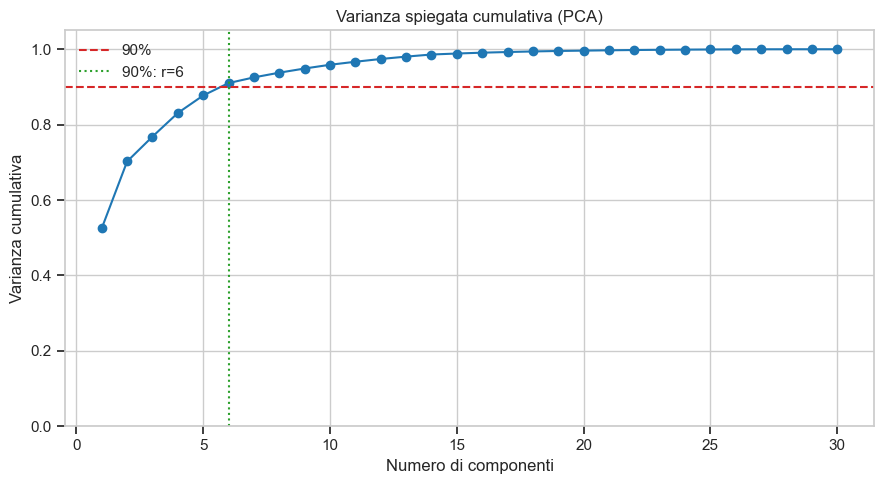
\includegraphics[width=\linewidth]{variance_cumulative.png}
\caption{Rango rappresentativo del 90\% della varianza}
\label{fig:PCA_variance_cumulative}
\end{figure}

\begin{figure}[htbp]
\centering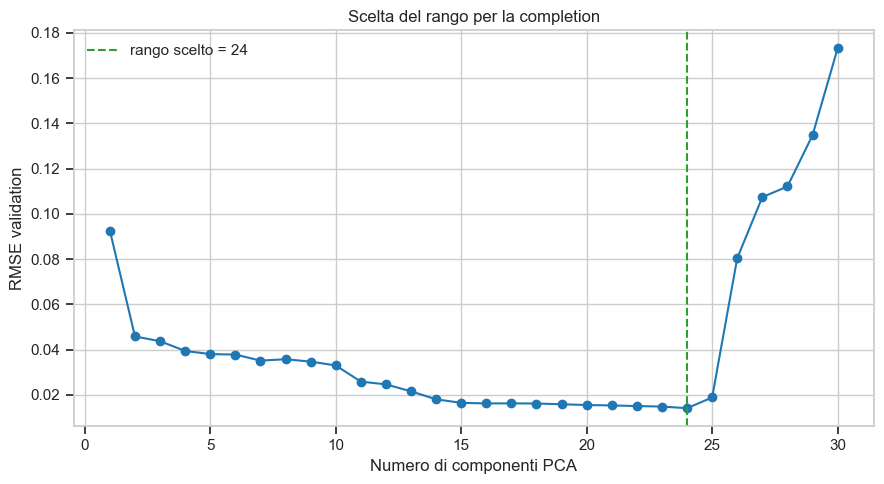
\includegraphics[width=\linewidth]{pca_rank_validation.png}
\caption{r=24 è il rango dello spazio trovato tramite PCA che minimizza RMSE}
\label{fig:PCA_rank_validation}
\end{figure}

\subsection{Regola PCA iterativa}
La PCA del notebook parte da $x^{(0)}$, ovvero uno spazio a rango 1 monodimensionale, che sostituisce le coordinate nascoste con $\mu$. Poi, per 30 iterazioni,
\[
\widetilde x^{(t+1)}=\mu+(x^{(t)}-\mu)P_r,\qquad
x^{(t+1)}_j=\begin{cases}x_j,&j\in\Obs_i,\\
\widetilde x^{(t+1)}_j,&j\in\Hidden_i.
\end{cases}
\]
Le coordinate osservate sono quindi ripristinate a ogni passo. Dopo l'ultima iterazione, 
la ricostruzione è limitata a $[0,1]$. 

\subsection{Regola SVD con adattamento sulle coordinate osservate}
La SVD calcola per ogni riga incompleta un vettore di coefficienti usando soltanto $\Obs_i=\{j:M_{ij}=1\}$:
\[
\widehat z_i=\arg\min_{z\in\R^r}
\left\|x_{i,\Obs_i}-\mu_{\Obs_i}-V_{r,\Obs_i}z\right\|_2^2
+\lambda\|z\|_2^2,\qquad\lambda=10^{-3}.
\]
Per $j\in\Hidden_i$ pone $\widehat x_{ij}=\mu_j+(V_r\widehat z_i)_j$; per $j\in\Obs_i$ conserva $x_{ij}$. Il piccolo $\lambda$ regolarizza il problema dei coefficienti latenti ed è distinto da $\alpha=1$ della Ridge supervisionata. Anche qui si applica clipping finale a $[0,1]$.

\subsection{Equivalenza a parità di completion rule}
Poiché PCA e SVD fattorizzano il medesimo $X_c$, le rispettive basi $V_r^{\rm PCA}$ e $V_r^{\rm SVD}$ individuano lo stesso sottospazio principale, eventualmente con segni o rotazioni ortogonali differenti. Se $V_r^{\rm PCA}=V_r^{\rm SVD}Q$ con $Q^{\mathsf T}Q=I$, allora i proiettori coincidono. Nella regola osservata-regolarizzata appena definita, il cambio di variabile $z'=Qz$ conserva sia il residuo sia la penalizzazione isotropa $\lambda\|z\|_2^2$. Ne segue la medesima ricostruzione anche sulle coordinate nascoste, a parità di media, rango, maschera, $\lambda$ e clipping.

Il notebook verifica esplicitamente tale affermazione per \emph{tutti} i ranghi 1-30 
su validation e test, passando alla stessa funzione di completion come vediamo in 
Figura \ref{fig:PCA_SVD_V_same_vectors}. Nell'esecuzione 
riprodotta, la massima differenza registrata nei proiettori, nelle predizioni sulle 
celle nascoste e negli RMSE è 0 alla precisione numerica riportata. Per esempio, con 
la procedura comune l'RMSE test è 0,045196 per entrambe le basi a $r=6$, e 0,023223 
a $r=24$.

\begin{figure}[htbp]
\centering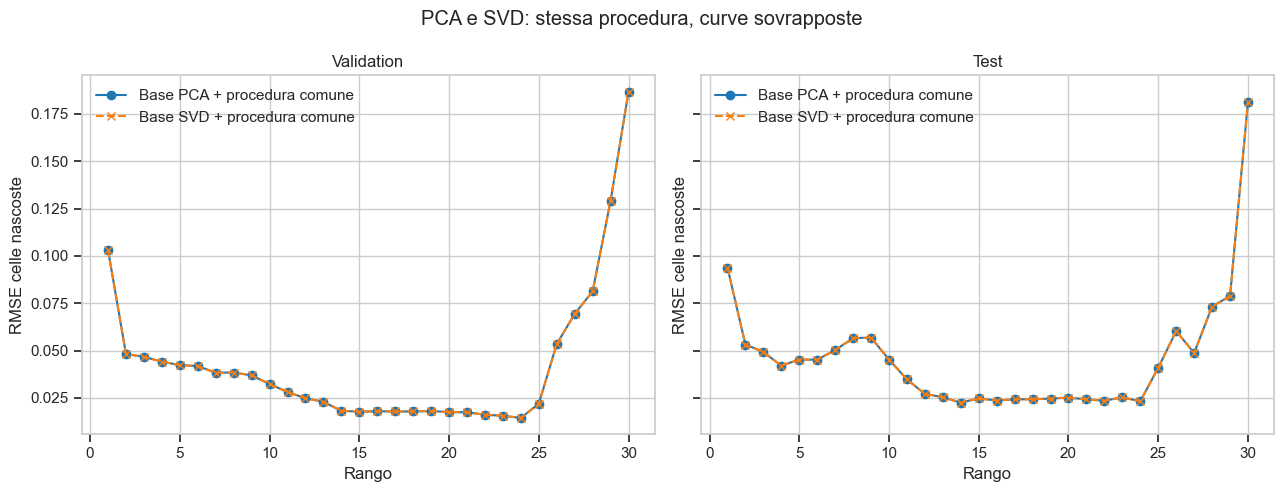
\includegraphics[width=\linewidth]{PCA_SVD_equivalence.png}
\caption{Performance uguali tra PCA e SVD alle quali viene applicata la stessa completion procedure.
Questo risultato è prevedibile dato che SVD è stata computata con lo stesso dataset usato per PCA ma
centrato.}
\label{fig:PCA_SVD_V_same_vectors}
\end{figure}

È importante reiterare che questa equivalenza è vera se viene utilizzata \emph{la stessa completion rule}. 
Nelle tabelle principali, PCA iterativa e SVD con adattamento regolarizzato usano regole 
diverse come visto in Figura \ref{fig:PCA_SVD_rank_validation}; piccole differenze di RMSE sono quindi coerenti con l'identità del sottospazio. 
Il fatto che la PCA sia centrata è essenziale: una SVD applicata alla matrice non centrata 
non avrebbe in generale le stesse direzioni della PCA qui utilizzata.

\begin{figure}[htbp]
\centering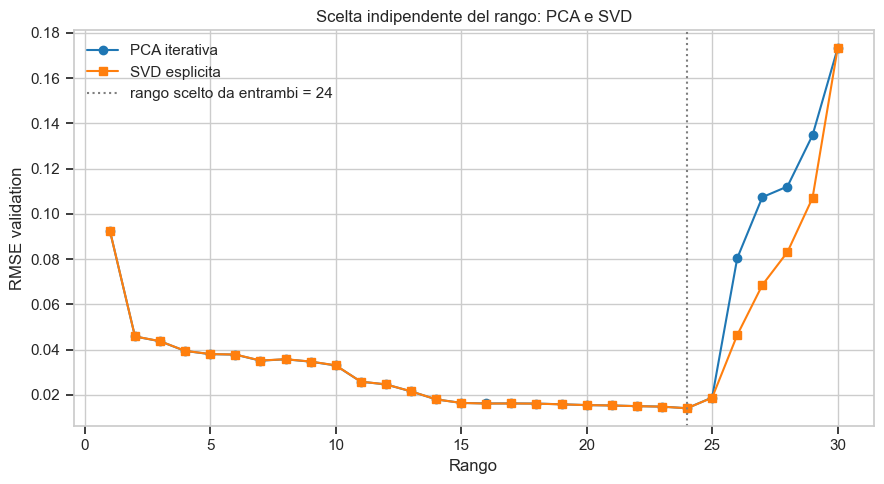
\includegraphics[width=\linewidth]{pca_svd_rank_validation.png}
\caption{Due completion rules diverse possono portare il RMSA di PCA e SVD a divergere anche se il loro spazio vettorile è uguale}
\label{fig:PCA_SVD_rank_validation}
\end{figure}

\section{Risultati principali e confronto tra rango 6 e rango 24}
Ricordiamo la dipperenza tra OLS matr/Ridge matr completo e complete-case:
\begin{itemize}
    \item \textbf{completo}: il modello è trainato sull'intero training set (anche se alcune entry sono NaN);
    \item \textbf{complete-case}: il modello è trainato sui soli oggetti completi.
\end{itemize}
\begin{table}[ht]
\centering\scriptsize
\caption{Tutti e nove i metodi sulla maschera principale: validation (74 celle) e test (50 celle). Rango 24 scelto su cinque maschere di validation; rango 6 fissato dal criterio descrittivo del 90\%.}
\label{tab:all-results}
\begin{tabular}{@{}lrrrrrr@{}}
\toprule
& \multicolumn{3}{c}{Validation} & \multicolumn{3}{c}{Test} \\
\cmidrule(lr){2-4}\cmidrule(l){5-7}
Metodo & RMSE & MAE & $R^2$ & RMSE & MAE & $R^2$ \\
\midrule
Media & 0,1867 & 0,1412 & 0,0536 & 0,1814 & 0,1417 & 0,0799 \\
OLS matr. completo & 0,0130 & 0,0082 & 0,9954 & 0,0231 & 0,0116 & 0,9851 \\
OLS matr. complete-case & 0,0140 & 0,0085 & 0,9947 & 0,0518 & 0,0171 & 0,9251 \\
Ridge matr. completo & 0,0127 & 0,0082 & 0,9956 & 0,0226 & 0,0122 & 0,9858 \\
Ridge matr. complete-case & 0,0144 & 0,0094 & 0,9944 & 0,0357 & 0,0162 & 0,9644 \\
PCA iterativa, $r=24$ & 0,0144 & 0,0096 & 0,9943 & 0,0234 & 0,0131 & 0,9847 \\
SVD esplicita, $r=24$ & 0,0144 & 0,0096 & 0,9943 & 0,0232 & 0,0131 & 0,9849 \\
PCA iterativa, $r=6$ & 0,0418 & 0,0312 & 0,9525 & 0,0451 & 0,0323 & 0,9430 \\
SVD esplicita, $r=6$ & 0,0418 & 0,0312 & 0,9524 & 0,0452 & 0,0323 & 0,9429 \\
\bottomrule
\end{tabular}
\end{table}

Sulla maschera principale del test, il minimo RMSE fra i nove metodi è ottenuto da Ridge 
matriciale completo (0,02255). La PCA e la SVD (con metodologie di completion diverse) a 
rango 24 sono vicine (0,02336 e 0,02322), mentre il rango 6 produce 0,04515 e 0,04520: 
quasi due volte l'errore dei rispettivi modelli a rango 24. Sulla validation principale 
il rapporto è circa 2,9. La scelta $r=6$ mantiene una forte compressione e il 91,03\% 
della varianza, ma scarta direzioni che in questo problema risultano utili a ricostruire 
le tre feature occultate. La quota di varianza globale non rappresentano una misura diretta 
dell'errore sulle celle nascoste.

\begin{figure}[htbp]
\centering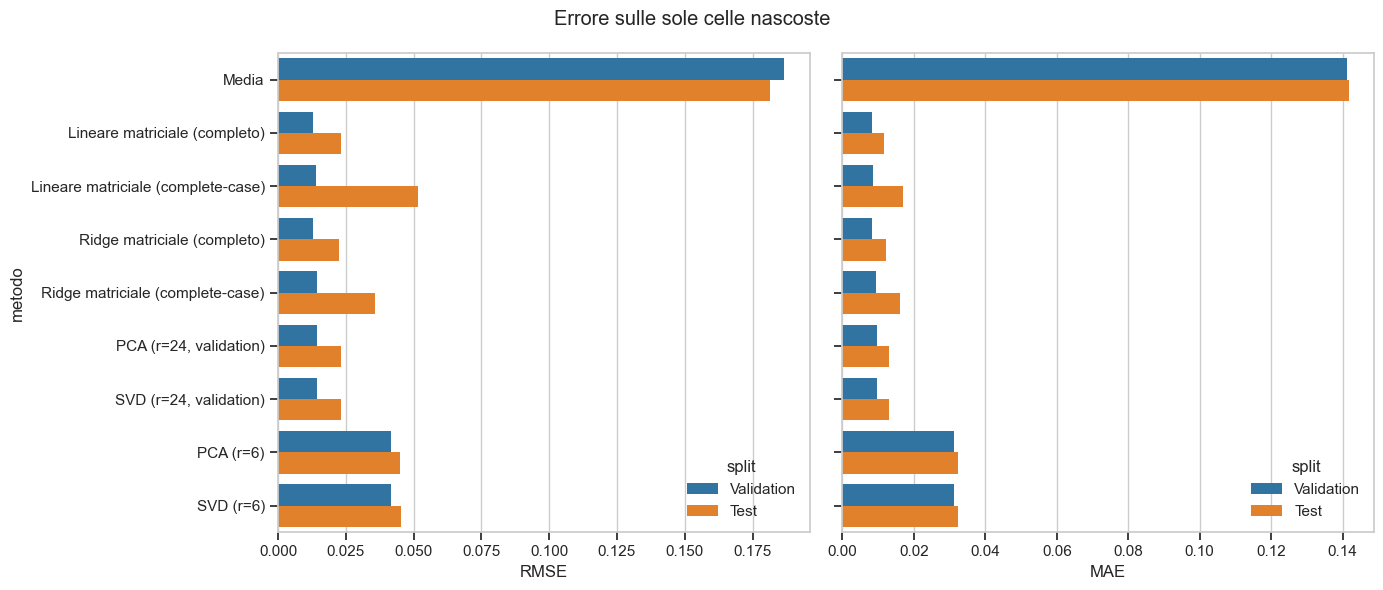
\includegraphics[width=.99\linewidth]{method_errors.png}
\caption{RMSE e MAE dei nove metodi sulle celle nascoste delle maschere principali.}
\label{fig:method-errors}
\end{figure}

\subsection{Errore per feature e un esempio di ricostruzione}
L'RMSE aggregato può nascondere difficoltà di completion per particolari features. Nel test,  
sono rappresentati 50 oggetti ma sono valutate solo 19 entry per \feat{mean\_radius}, 17 per \feat{mean\_concavity} e 14 per 
\feat{worst\_radius} a causa della maschera. La Tabella \ref{tab:feature-errors} mostra i valori per ciascun 
metodo. 

\begin{table}[ht]
\centering\small
\caption{RMSE test per feature nascosta.}
\label{tab:feature-errors}
\begin{tabular}{@{}lrrr@{}}
\toprule
Metodo & \feat{mean\_radius} & \feat{mean\_concavity} & \feat{worst\_radius} \\
\midrule
Media & 0,1745 & 0,1705 & 0,2023 \\
OLS matr. completo & 0,0026 & 0,0391 & 0,0060 \\
OLS matr. complete-case & 0,0030 & 0,0884 & 0,0080 \\
Ridge matr. completo & 0,0031 & 0,0379 & 0,0076 \\
Ridge matr. complete-case & 0,0047 & 0,0600 & 0,0120 \\
PCA iterativa, $r=24$ & 0,0042 & 0,0393 & 0,0067 \\
SVD esplicita, $r=24$ & 0,0041 & 0,0391 & 0,0067 \\
PCA iterativa, $r=6$ & 0,0307 & 0,0612 & 0,0380 \\
SVD esplicita, $r=6$ & 0,0309 & 0,0612 & 0,0381 \\
\bottomrule
\end{tabular}
\end{table}

\begin{table}[ht]
\centering\small
\caption{Esempio di completion su due celle della medesima riga test. I valori veri sono mostrati solo per verificare l'errore.}
\label{tab:example}
\begin{tabular}{@{}lrrrrrr@{}}
\toprule
Feature & Vero & Media & OLS comp.case. & Ridge comp.case. & PCA $r=24$ & SVD $r=24$ \\
\midrule
\feat{mean\_concavity} & 0,0857 & 0,2082 & 0,0890 & 0,0840 & 0,0986 & 0,0988 \\
\feat{worst\_radius} & 0,1967 & 0,2969 & 0,1994 & 0,1990 & 0,1946 & 0,1948 \\
\bottomrule
\end{tabular}
\end{table}

\section{Analisi di sensibilità presenti nel notebook}
\subsection{Cambiare il gruppo di feature target}
Sono stati confrontati due gruppi di feature, uno che chiamiamo ``distribuito'' 
$\{\feat{mean\_radius},\feat{mean\_concavity},\feat{worst\_radius}\}$ ovvero quello analizzato fin ora
e un gruppo che chiamiamo ``raggio'' $\{\feat{mean\_radius},\feat{radius\_error},\feat{worst\_radius}\}$. 
Entrambe le prove generano una nuova maschera test (con seed fissato per riproducibilità) con 47 celle 
nascoste; per le varianti mascherate dei regressori si genera anche una nuova maschera train 
(con seed fissato per riproducibilità). I regressori sono riaddestrati sui tre target appropriati e sulle 
altre 27 feature come predittori comuni; Queste prove cambiano quindi il gruppo di feature da completare.

\begin{table}[ht]
\centering\small
\caption{RMSE test con due gruppi di feature occultate.}
\label{tab:patterns}
\begin{tabular}{@{}lrr@{}}
\toprule
Metodo & Gruppo distribuito & Famiglia del raggio \\
\midrule
Media & 0,1770 & 0,1738 \\
OLS matr. completo & 0,0241 & 0,0229 \\
OLS matr. complete-case & 0,0372 & 0,0151 \\
Ridge matr. completo & 0,0206 & 0,0185 \\
Ridge matr. complete-case & 0,0273 & 0,0236 \\
PCA iterativa, $r=24$ & 0,0246 & 0,0301 \\
SVD esplicita, $r=24$ & 0,0245 & 0,0301 \\
PCA iterativa, $r=6$ & 0,0523 & 0,0501 \\
SVD esplicita, $r=6$ & 0,0523 & 0,0501 \\
\bottomrule
\end{tabular}
\end{table}

\begin{figure}[htbp]
\centering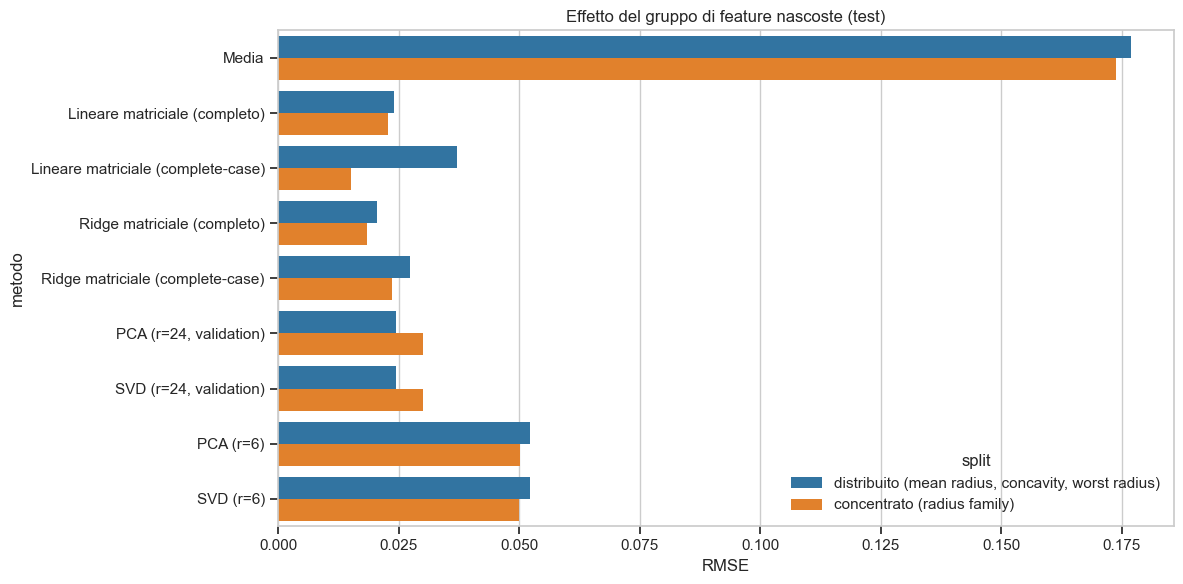
\includegraphics[width=.97\linewidth]{feature_group_sensitivity.png}
\caption{Sensibilità dell'RMSE al gruppo di feature nascoste. Figura originale del notebook.}
\label{fig:patterns}
\end{figure}

\subsection{Cambiare la probabilità di occultamento}
Mantenendo le tre feature target principali e i modelli già stimati, il notebook valuta 
$p=10\%,30\%,50\%,70\%$, ovvero la probabilità di occultamento delle feature target, 
con seed fissato. I dati di Figura~\ref{tab:all-results} sono stati computati cambiano il seed della maschera,
quindi i risultati del gruppo ``distribuito'' sono leggermente diversi da quelli della Figura~\ref{fig:method-errors}.

\begin{table}[H]
\centering\scriptsize
\caption{RMSE test per probabilità (feature nascoste) di occultamento nelle tre colonne target.}
\label{tab:probability}
\begin{tabular}{@{}lrrrr@{}}
\toprule
Metodo & 10\% (17) & 30\% (49) & 50\% (91) & 70\% (127) \\
\midrule
Media & 0,1722 & 0,1697 & 0,1713 & 0,1761 \\
OLS matr. completo & 0,0087 & 0,0185 & 0,0163 & 0,0174 \\
OLS matr. complete-case & 0,0092 & 0,0203 & 0,0169 & 0,0341 \\
Ridge matr. completo & 0,0089 & 0,0182 & 0,0160 & 0,0172 \\
Ridge matr. complete-case & 0,0094 & 0,0181 & 0,0153 & 0,0243 \\
PCA iterativa, $r=24$ & 0,0100 & 0,0233 & 0,0201 & 0,0195 \\
SVD esplicita, $r=24$ & 0,0098 & 0,0233 & 0,0200 & 0,0194 \\
PCA iterativa, $r=6$ & 0,0268 & 0,0447 & 0,0415 & 0,0457 \\
SVD esplicita, $r=6$ & 0,0267 & 0,0447 & 0,0415 & 0,0457 \\
\bottomrule
\end{tabular}
\end{table}

\begin{figure}[H]
\centering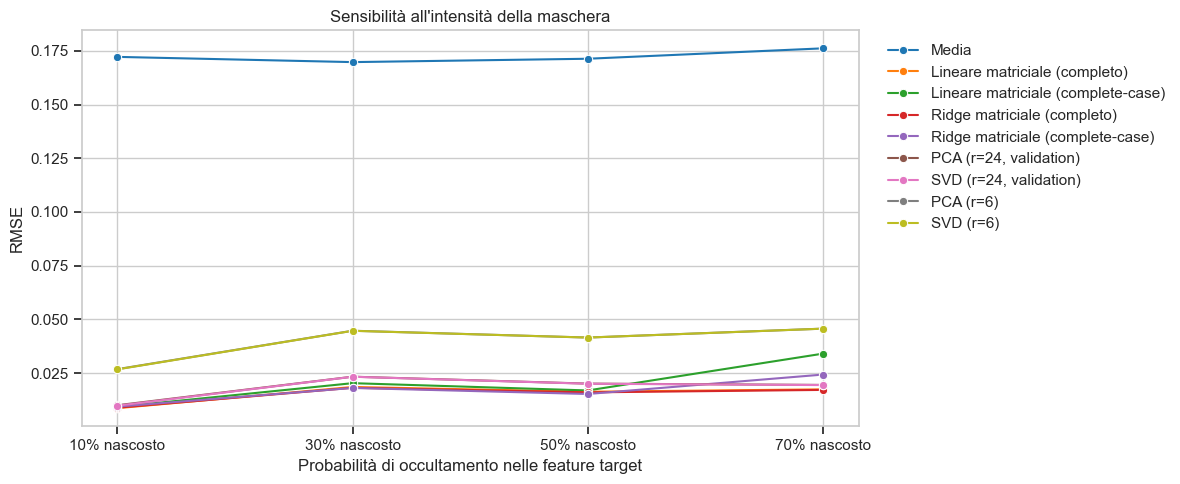
\includegraphics[width=.98\linewidth]{mask_probability_sensitivity.png}
\caption{RMSE dei nove metodi per diverse probabilità di mascheramento delle feature target.}
\label{fig:probability}
\end{figure}

\section{Conclusioni}
\textbf{Quale informazione rende prevedibili i valori nascosti?}
Le 27 feature sempre osservate contengono misure correlate di dimensione
e forma: i regressori ne sfruttano la ridondanza e PCA/SVD stimano i
coefficienti latenti dalle coordinate rimaste visibili. Sul test
principale la media ha RMSE $0{,}1814$; il minimo fra i nove metodi è Ridge matriciale (completo), 
con RMSE $0{,}0226$. PCA/SVD a rango 24 ottengono circa $0{,}023$, il rango 6 conserva il 91,03\% 
della varianza, ma perde direzioni utili per questa completion. Le tre colonne non
sono ugualmente facili da ricostruire: \feat{mean\_concavity} resta la
più difficile anche se la completion è ad ogni modo di qualità. 

Questi risultati riguardano il test set principale. 
Ripetere split e maschere, e occultare più colonne,
permetterebbe di stimare la variabilità e di capire quanto la
prestazione dipenda dal protocollo scelto. Questo approccio tuttavia non è stato
usato.

\section{Required check: SVD troncata e proiettori}
\label{sec:required-check}
Il controllo richiesto dalla consegna è eseguito al termine del notebook
sulla matrice del training centrata, $X_c=X_{\rm train}-\mathbf{1}\mu^{\mathsf T}$, dove $\mu$ contiene 
le medie delle feature del training.
Si riutilizza la SVD $X_c=U\Sigma V^{\mathsf T}$ e si fissa $r=6$,
senza selezionare il rango sul test. Definiamo
\[
X_r=U_r\Sigma_rV_r^{\mathsf T},\qquad
P_r^{(s)}=U_rU_r^{\mathsf T}\in\R^{n\times n},\qquad
P_r^{(f)}=V_rV_r^{\mathsf T}\in\R^{d\times d}.
\]
Il primo proiettore agisce nello spazio delle osservazioni, il secondo nello
spazio delle feature. La verifica confronta le quattro forme
\[
P_r^{(s)}X_c\approx X_cP_r^{(f)}\approx
P_r^{(s)}X_cP_r^{(f)}\approx X_r.
\]

\begin{table}[H]
\centering\small
\caption{Required check con $r=6$: confronto di tutte le coppie di ricostruzioni.
Lo scarto relativo è $\frac{\|A-B\|_F}{\|X_r\|_F}$; il massimo è calcolato sulle singole celle.}
\label{tab:required-check}
\begin{tabular}{@{}lrrr@{}}
\toprule
Confronto $A$ vs $B$ & $\|A-B\|_F$ & Scarto relativo & Max. assoluto \\
\midrule
$P_r^{(s)}X_c$ vs $X_cP_r^{(f)}$ & $2{,}287\cdot10^{-14}$ & $1{,}406\cdot10^{-15}$ & $2{,}304\cdot10^{-15}$ \\
$P_r^{(s)}X_c$ vs $P_r^{(s)}X_cP_r^{(f)}$ & $1{,}473\cdot10^{-14}$ & $9{,}059\cdot10^{-16}$ & $1{,}332\cdot10^{-15}$ \\
$P_r^{(s)}X_c$ vs $X_r$ & $1{,}524\cdot10^{-14}$ & $9{,}371\cdot10^{-16}$ & $1{,}332\cdot10^{-15}$ \\
$X_cP_r^{(f)}$ vs $P_r^{(s)}X_cP_r^{(f)}$ & $1{,}824\cdot10^{-14}$ & $1{,}122\cdot10^{-15}$ & $2{,}331\cdot10^{-15}$ \\
$X_cP_r^{(f)}$ vs $X_r$ & $1{,}955\cdot10^{-14}$ & $1{,}202\cdot10^{-15}$ & $2{,}331\cdot10^{-15}$ \\
$P_r^{(s)}X_cP_r^{(f)}$ vs $X_r$ & $1{,}355\cdot10^{-14}$ & $8{,}331\cdot10^{-16}$ & $7{,}772\cdot10^{-16}$ \\
\bottomrule
\end{tabular}
\end{table}

Tutti i confronti superano gli assert con tolleranze assoluta e relativa
$10^{-10}$. Il massimo scarto per cella è circa $2{,}33\cdot10^{-15}$:
le quattro forme coincidono entro gli errori di arrotondamento numerico.

\begin{table}[H]
\centering\small
\caption{}
\label{tab:required-projectors}
\begin{tabular}{@{}lrrrr@{}}
\toprule
Proiettore & $m$ & Rango & $\|P^2-P\|_F$ & $\|P-I_m\|_F$ \\
\midrule
$P_r^{(s)}$ (osservazioni) & 426 & 6 & $2{,}117\cdot10^{-15}$ & $20{,}493902$ \\
$P_r^{(f)}$ (feature) & 30 & 6 & $3{,}398\cdot10^{-15}$ & $4{,}898979$ \\
\bottomrule
\end{tabular}
\end{table}

\textbf{Perché i proiettori non sono l'identità?}
\begin{proof}
Formalmente la motivazione per il quale l'equazione 
\[
P_r^{(s)}X_c= X_cP_r^{(f)}=
P_r^{(s)}X_cP_r^{(f)}= X_r
\]
è soddisfatta è che possiamo riscrivere il tutto come
\[
P_r^{(s)}U\Sigma V^T=U\Sigma V^TP_r^{(f)}=
P_r^{(s)}U\Sigma V^TP_r^{(f)}= X_r
\]
è importante a questo punto un osservazione: $U^T_rU=\begin{bmatrix} I_r & 0 \end{bmatrix}$ e 
$V^T_rV=\begin{bmatrix} I_r\\0\end{bmatrix}$. Questo accade perchè possiamo scrivere $U$ distinguendo i 
vettori di base principali dagli altri, quindi $U=\begin{bmatrix}U_r, U_{\text{rest}}\end{bmatrix}$, quindi 
$U^T_rU_r=U_r^T\begin{bmatrix} U_r\;\;U_\text{rest}\end{bmatrix}=\begin{bmatrix} U^T_rU_r\;\;\;U^T_rU_\text{rest}\end{bmatrix}
=\begin{bmatrix} I_r & 0 \end{bmatrix}$ 
e $U_r^TU_\text{rest}=0$ perchè i vettori sono ortonormali, quindi i prodotti scalari 
danno 0. Con un ragionamento analogo si ottiene $V^T_rV=\begin{bmatrix} I_r\\0\end{bmatrix}$. Quindi:
\[
\begin{aligned}
    P_r^{(s)}X_c&
    =U_rU^T_rU\Sigma V^T\\&
    =U_r\begin{bmatrix} I_r & 0 \end{bmatrix}\Sigma V^T\\&
    =U_r\Sigma_rV_r^T=X_r
\end{aligned}
\]
e
\[
\begin{aligned}
    X_cP_r^{(f)}
    &=U\Sigma V^TV_rV_r^T\\
    &=U\Sigma\begin{bmatrix}I_r\\0\end{bmatrix}V_r^T\\
    &=U_r\Sigma_rV_r^T
    =X_r
\end{aligned}
\]
infine possiamo scrivere \[P_r^{(s)}X_cP_r^{(f)} = X_rP_r^{(f)}=U_r\Sigma_rV_r^TV_rV_r^T\]
ma $V_r^TV_r=I_r$, quindi otteniamo \[P_r^{(s)}X_cP_r^{(f)}=U_r\Sigma_rV_r^T=X_r\]
il che dimostra che tutte e quattro le forme coincidono, ovvero
\[
P_r^{(s)}X_c= X_cP_r^{(f)}=
P_r^{(s)}X_cP_r^{(f)}= X_r.
\]
\end{proof}

\section*{Fonti e riproducibilità}
I numeri e le figure derivano dall'esecuzione salvata di
\nolinkurl{completion_breast_cancer_matrix.ipynb}. Le tabelle supplementari
sono ricostruite da \nolinkurl{report_assets/build_report_data.py};
i CSV in \nolinkurl{report_assets/} conservano i valori non arrotondati. 
Tutte le metriche si riferiscono alla scala normalizzata $[0,1]$.
\begin{landscape}
\begin{figure}[p]
\centering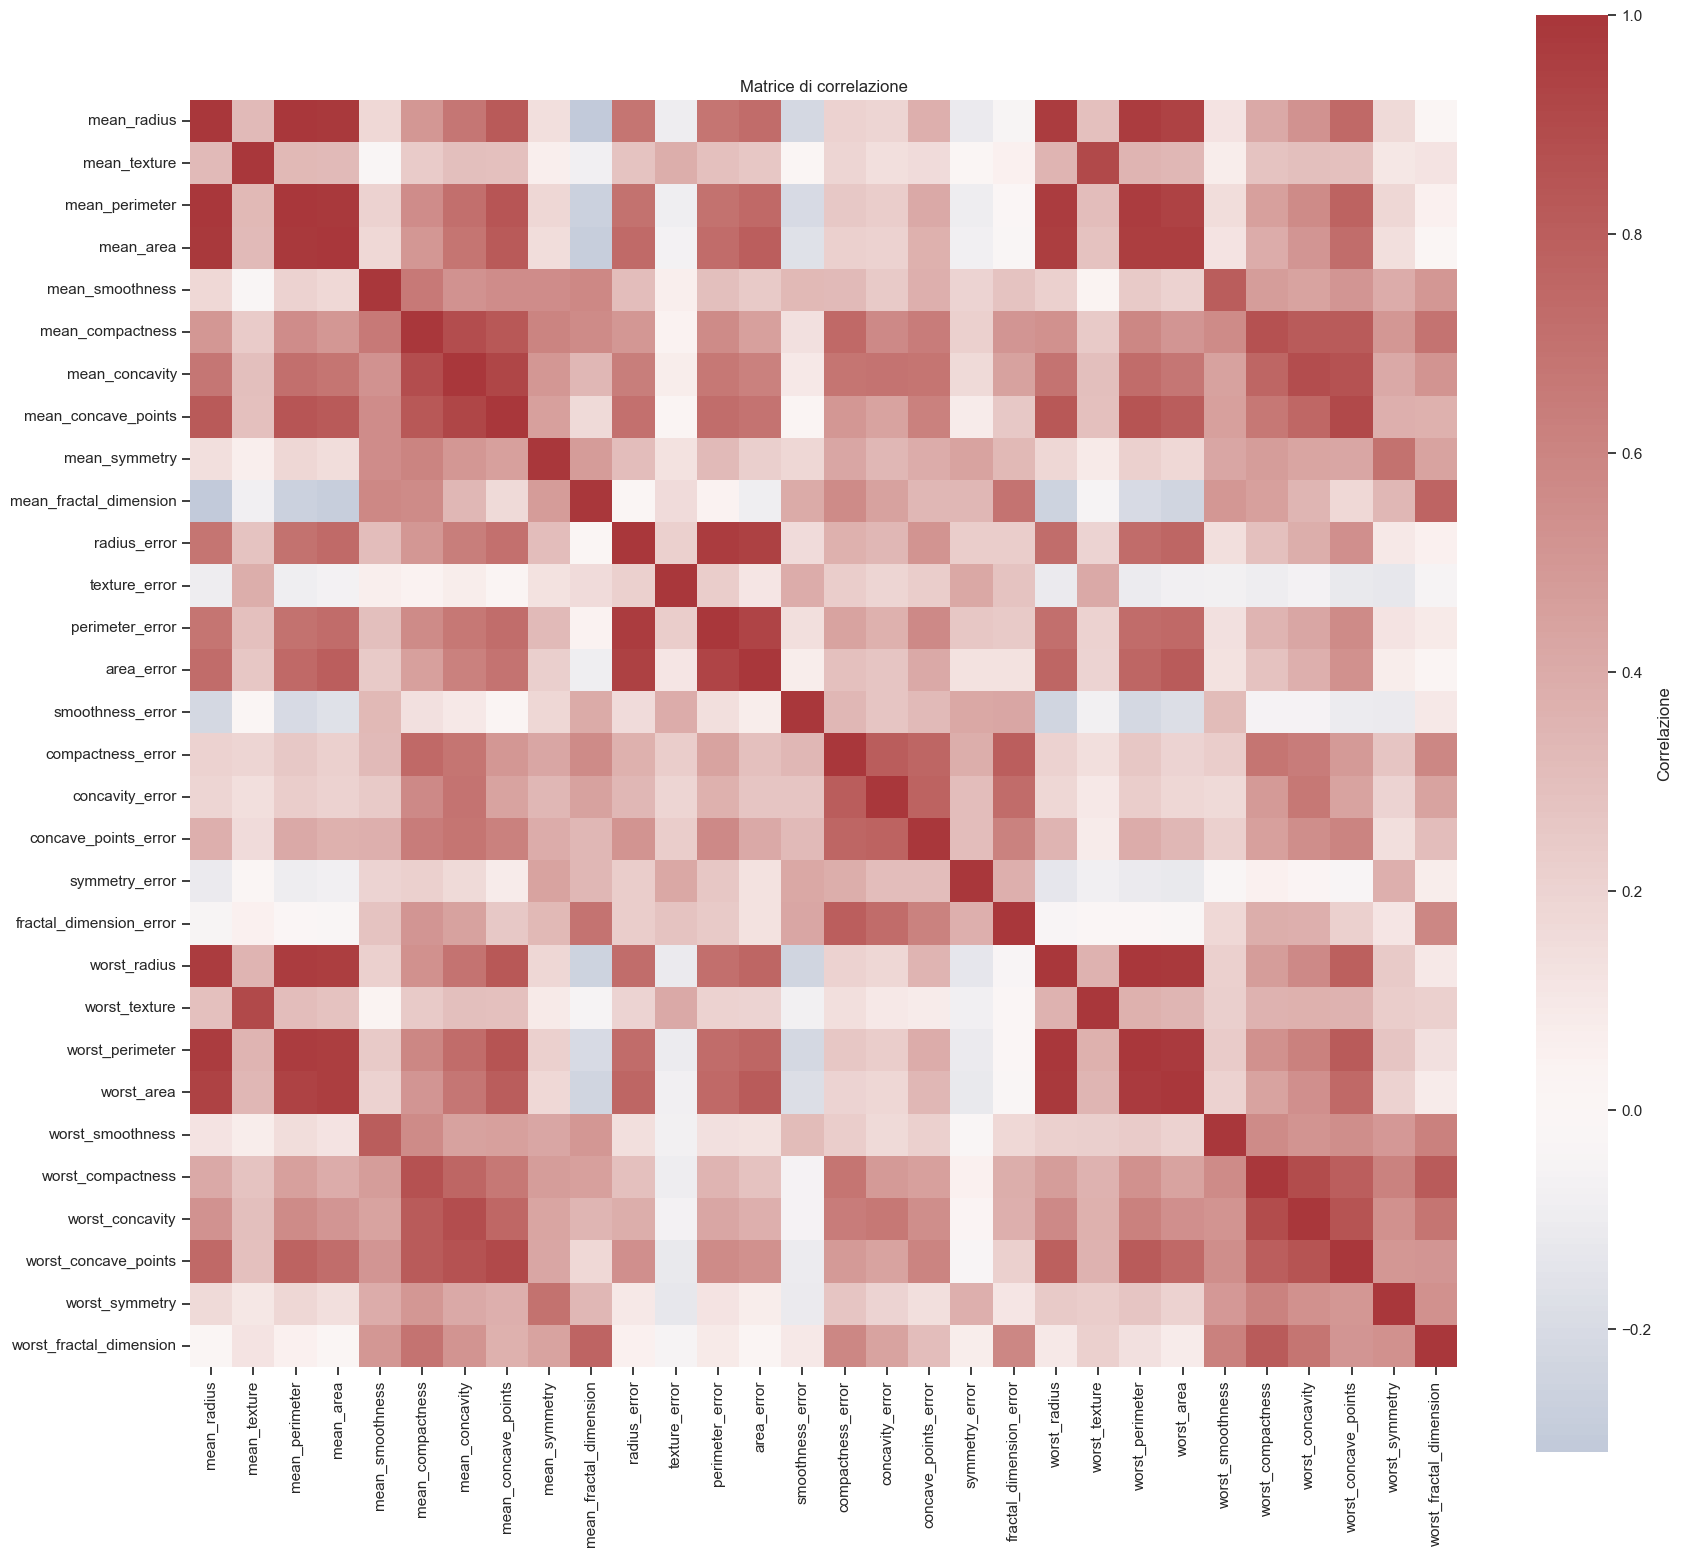
\includegraphics[width=\linewidth,keepaspectratio]{feature_correlations.png}
\caption{Correlazioni fra le 30 feature della matrice normalizzata.
I blocchi di colore più intenso mostrano la ridondanza sfruttata
dai metodi di completion;}
\label{fig:correlations}
\end{figure}
\end{landscape}

\clearpage
\appendix
\section{Interazioni con l'AI}
L'approccio con AI è stato di tipo agent-oriented. Oltre le query eseguite sono stati usati anche i vari
comandi messi a disposizione dai tool per la scelta dei modelli più appropriati, impostare goal, condividere files, ...
Il contesto degli agenti è sempre lo stesso, l'intero accesso alla cartella contenente notebook, richiesta dell'homework e
il libro di testo vincolato ai soli primi quattro capitoli (per coerenza nei formalismi).

\begin{enumerate}
\item \textbf{Prima struttura del notebook.}
\emph{Domanda:} Devo consegnare il progetto descritto in "homework\_ch1\_4\_completion 1.pdf".

La mia idea è quella di sfruttare il dataset breast\_cancer di scikitlearn. Le nozioni teoriche per supportare il problema si trovano in "CompletionAgent\_1.0.pdf".

Produci un notebook ricco di descrizioni dettagliate riguardo i passi intrapresi e le motivazioni in italiano e con anche definizioni tecniche.

Struttura del notebook:

- Importazione della matrice nxd.

- Proponi un analisi della matrice prodotta, quindi media, stdandard deviation, min, max.

- Plot della correlation matrix.

- Dividi la matrice in Training, Validation e Test set (75,15,15). Normalizza il training set.

- Su Validation set e Test set introduci una maschera M in grado di nascondere alcune entry. Fai in modo che è possibile controllare la matrice. È importante 
introdurre la possibilità di gestire la percentuale di features nascoste e quali features sono soggette alla maschera.

- Proponi un semplice mean completion rule (baseline), ovvere sostituisci il valore non osservato con il valore della media di tale feature (ovvero la media della colonna).

- Proponi una nuova completion rule che sfrutta la regressione lineare.

- Confronta i risultati ottenuti dalla baseline e dalla linear regression.

- Riemi ora i dati mancanti tramite media computa PCA e tramite la low-dimension structure fai completion delle feature nascoste.

Produci plot, tabelle e usa strumenti di visualizzazione che ritieni appropriati per analizzare i dati, relazioni e qualità dei modelli.
\emph{Esito:} L'agente ha prodotto un notebook di disceta qualità. È inutile nascondere che sono state necessarie correzioni
e aggiunte, come ad esempio nel caso della scelta del rango della PCA dato che non è stato esplicitato un criterio specifico nella mia query.

\item \textbf{Prima revisione del report.}
\emph{Domanda:} Analizza il notebook "completion\_breast\_cancer\_completion.ipynb", verifica problemi nella metodologia, struttura o 
incoerenza di possibili risultati. Verifica che non sono presenti ridondanze. Proponi migliorie se necessarie
\emph{Esito:} Questa query è stata eseguita in diverse fasi durante la produzione del notebook. Ha proposto migliorie
 e/o errori tecnici. Il progetto è stato ritenuto da me completato quando sono stato soddisfatto della qualità del notebook e l'agente
 ha proposto solo migliorie marginali. Nota che questa tipologia di query (analisi del lavoro prodotto) sarebbe potuta essere abusata
 tramite il comando goal, che avrebbe potuto portare a una revisione infinita del notebook e di conseguenza ad un consumo smisurato di token. 
 Ho quindi deciso di non abusare di questo comando e di limitarmi a una sola revisione finale. 

\item \textbf{Completo vs Complete case.}
\emph{Domanda:} Per i modelli OLS e Ridge aggiungi una variante trainata su un dataset composto solo dagli oggetti completamente osservati 
ovver quelli con tutti i valori disponibili (nessuna entry mancante nella matrice). Aggiungi questo modello nei vari 
confronti (tabelle, plot) del notebook.
\emph{Esito:} L'agente ha prodotto risultati di qualità. In questo caso è stata necessaria solo una revisione del lavoro dato
prodotto dall'agente data la qualità del lavoro prodotto.
\end{enumerate}

\end{document}
